\begin{frame}
\frametitle{The FF method}
%\beamercite{CMS-NOTE-2018-257}

\manip How many jets are mis-identified as \tauh? (fake taus)

\end{frame}

\begin{frame}
\frametitle{The FF method: principle}
%\beamercite{CMS-NOTE-2018-257}
\begin{center}
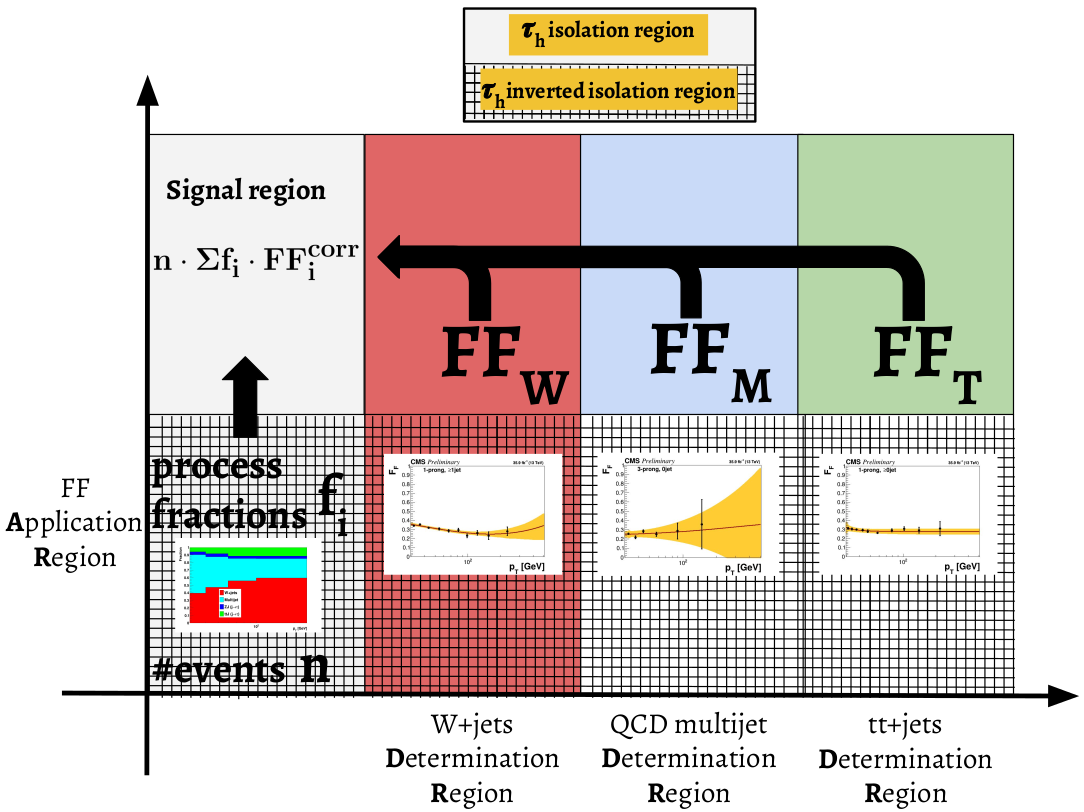
\includegraphics[width=\graphw,height=\graphh,keepaspectratio]{\PhDthesisdir/tex/slides/HTT_analysis/bg_estimations/FF_method/FF_ppe-Fig1a-AN-2018-257.png}
\end{center}
\end{frame}

\begin{frame}
\frametitle{The FF method: isolation cuts}
%\beamercite{CMS-NOTE-2018-257}

\begin{minipage}[c]{.45\textwidth}
For \tauh,
\begin{itemize}
\item iso = Tight MVA-iso
\item anti-iso = (VLoose \& not Tight)% MVA-iso
\end{itemize}

\manip AR very pure in events with fake taus.
\manip Impurities from actual \tauh\ decays are very low (less than few \%, can be up to \SI{20}{\%} close to \Zboson\ boson mass peak)
\end{minipage}
\hfill
\begin{minipage}[c]{.45\textwidth}
\begin{center}
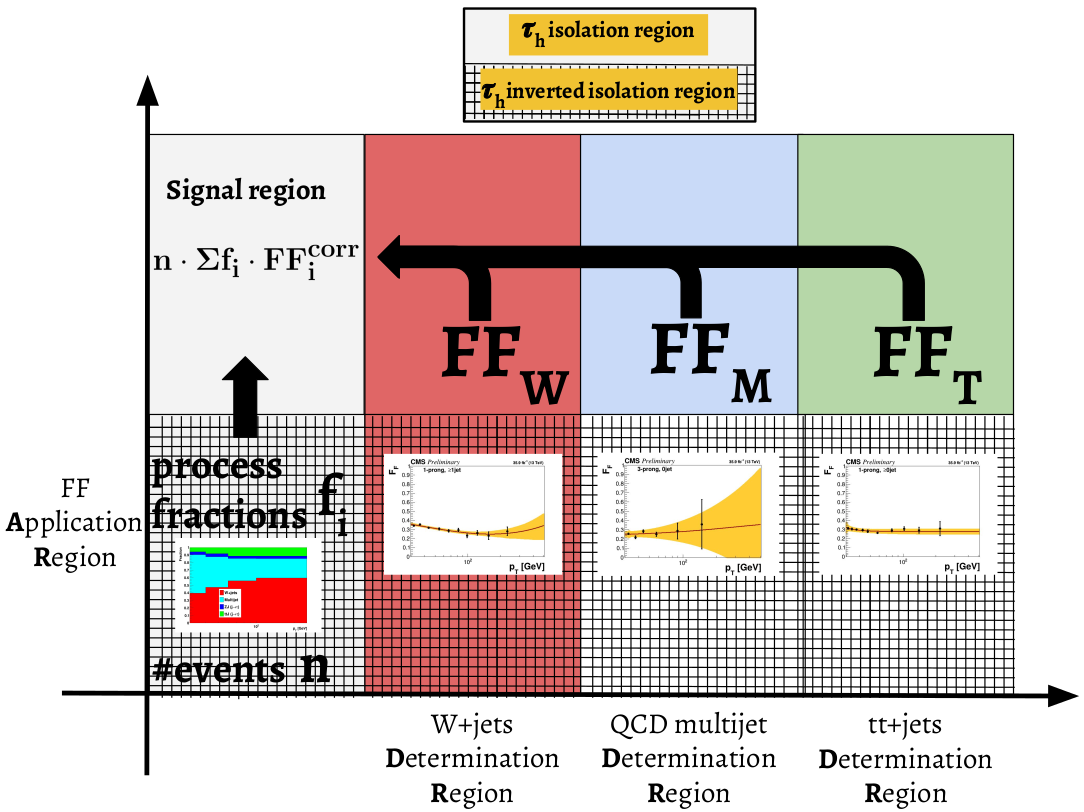
\includegraphics[width=\linewidth,height=\graphh,keepaspectratio]{\PhDthesisdir/tex/slides/HTT_analysis/bg_estimations/FF_method/FF_ppe-Fig1a-AN-2018-257.png}
\end{center}
\end{minipage}

\end{frame}

\begin{frame}
\frametitle{The FF method: obtaining amount of fakes}
%\beamercite{CMS-NOTE-2018-257}

\begin{minipage}[c]{.45\textwidth}
\manip One DR for each process giving fakes:\\$\Wboson+\text{jets}$, QCD multijets, $\quarkt\antiquarkt+\text{jets}$.

\manip For each range of kinematic variables:\\
\qquad $\pT$, $\eta$, nb. of hadrons, jet multiplicity...
%TODO , $m_{\tau\tau}$\todo{?}.
\begin{equation*}
\boxed{n_{j\to\tauh} = n_\text{AR}\sum_i f_i \cdot \mathrm{FF}_i}
\end{equation*}

\manip $f_i$ and $\mathrm{FF}_i$ are then functions of the kinematic variables.
\end{minipage}
\hfill
\begin{minipage}[c]{.45\textwidth}
\begin{center}
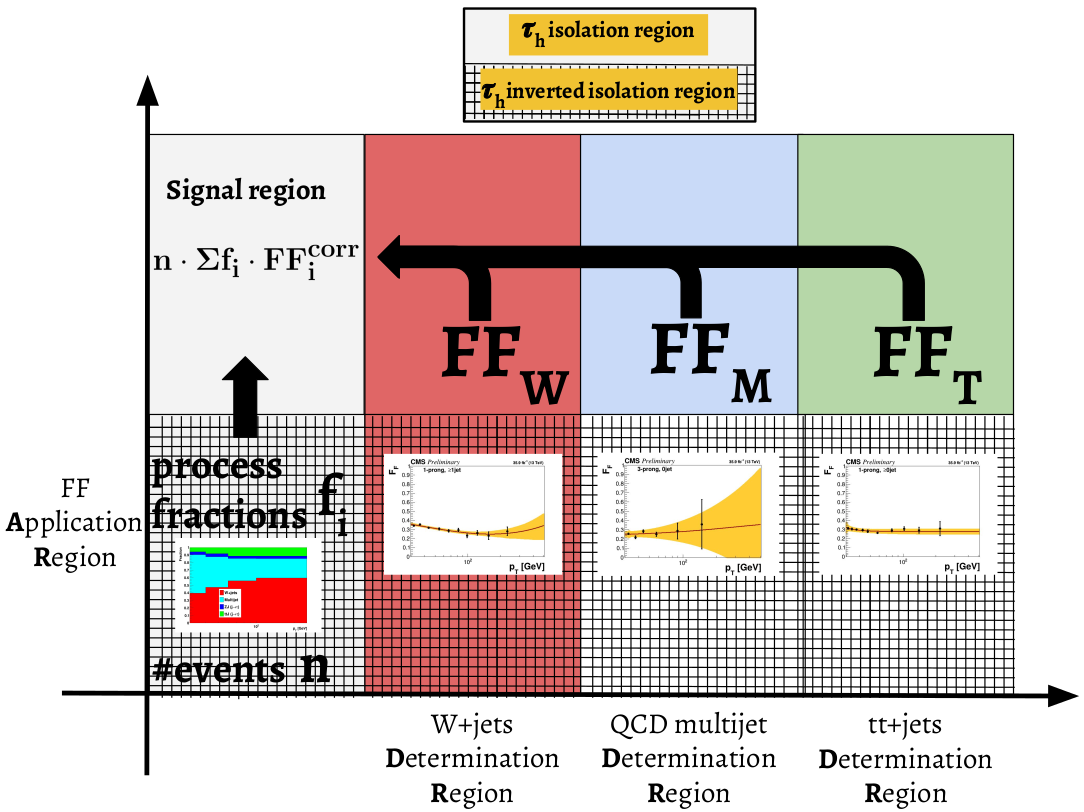
\includegraphics[width=\linewidth,height=\graphh,keepaspectratio]{\PhDthesisdir/tex/slides/HTT_analysis/bg_estimations/FF_method/FF_ppe-Fig1a-AN-2018-257.png}
\end{center}
\end{minipage}
\end{frame}

\begin{frame}
\frametitle{The FF method: determination regions definitions}
%\beamercite{CMS-NOTE-2018-257}

\begin{block}{QCD multijets}
Same as SR, except:
\begin{itemize}
\item same signs for $L_1$ and $L_2$ electric charges (opposite signs in the SR).
\end{itemize}
\end{block}

\pause\vfill

\begin{block}{$\Wboson+\text{jets}$}
Same as SR, except:
\begin{itemize}
\item transverse mass $m_T^{(\ell)}>\SI{70}{GeV}$ ($m_T^{(\ell)}<\SI{50}{GeV}$ in the SR);
\item no \quarkb-jet (allowed in the SR).
\end{itemize}
\end{block}

\pause\vfill

\begin{block}{$\quarkt\antiquarkt+\text{jets}$}
Estimation from simulated samples.
\end{block}

\end{frame}

\begin{frame}
\frametitle{The FF method: fine $\mathit{FF}$}
%\beamercite{CMS-NOTE-2018-257}

\manip Maybe the DR are not \SI{100}{\%} pure in terms of process-of-interest.

\manip To ensure purity, slighlty change $\mathrm{FF}_i$ definition
\begin{equation*}
\mathrm{FF}_i = \frac{n_\text{iso}}{n_\text{anti-iso}}
\rightsquigarrow
\mathrm{FF}_i = \frac{n_\text{iso} - n_\text{iso}^\text{rest}}{n_\text{anti-iso} - n_\text{anti-iso}^\text{rest}}
\end{equation*}
\begin{center}
{\small $n_x^\text{rest}$ = impurity of backgrounds other than from the process-of-interest in the DR, MC-driven.}
\end{center}
\end{frame}

\begin{frame}
\frametitle{The FF method}
%\beamercite{CMS-NOTE-2018-257}
\begin{center}
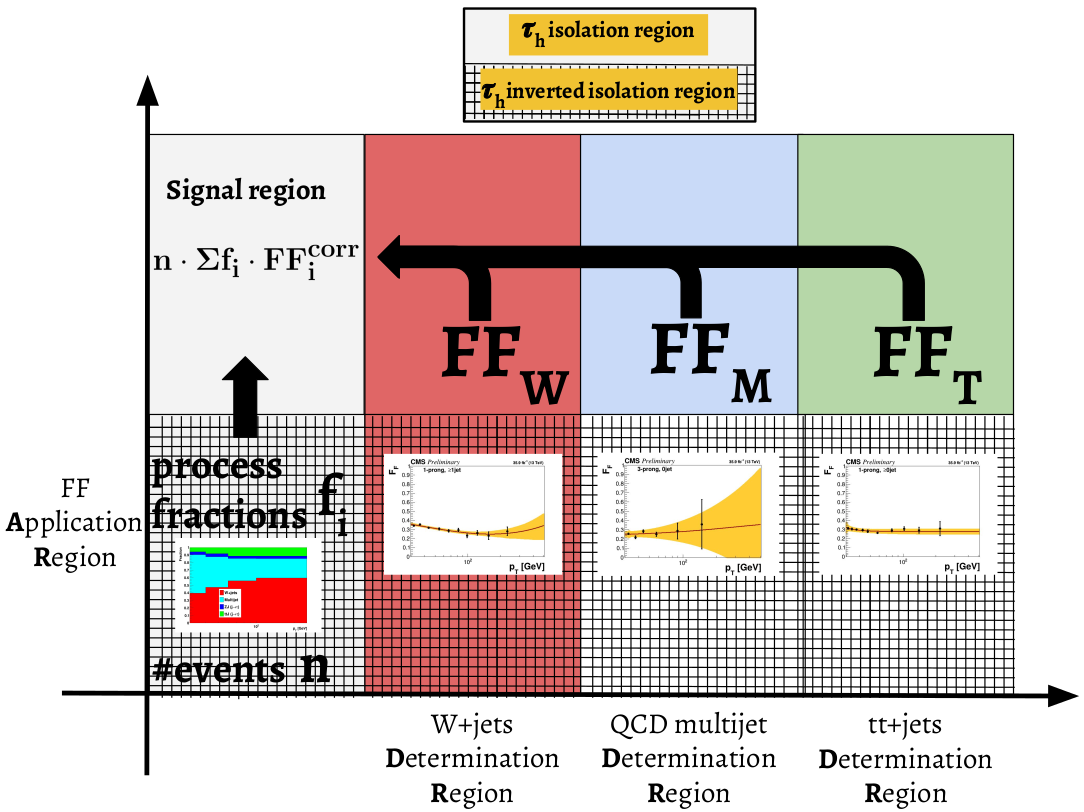
\includegraphics[width=\graphw,height=\graphh,keepaspectratio]{\PhDthesisdir/tex/slides/HTT_analysis/bg_estimations/FF_method/FF_ppe-Fig1a-AN-2018-257.png}
\end{center}
\end{frame}